%! Author = denis
%! Date = 09/08/2026


\begin{frame}{Tempo contínuo e tempo discreto}
    \begin{itemize}
        \item Sinal analógico
        \item Sinal digital
    \end{itemize}

    \begin{columns}[T]
        \begin{column}{0.48\textwidth}
            \centering
            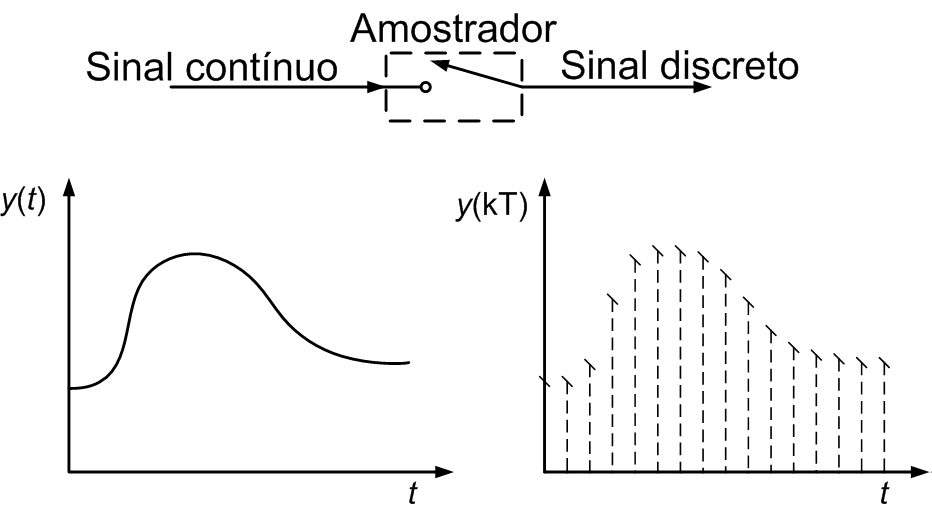
\includegraphics[width=\textwidth]{images/tempo.png}

            \vspace{0.2cm}
            \textbf{Amostragem de sinal}
        \end{column}

        \begin{column}{0.4\textwidth}
            \centering
            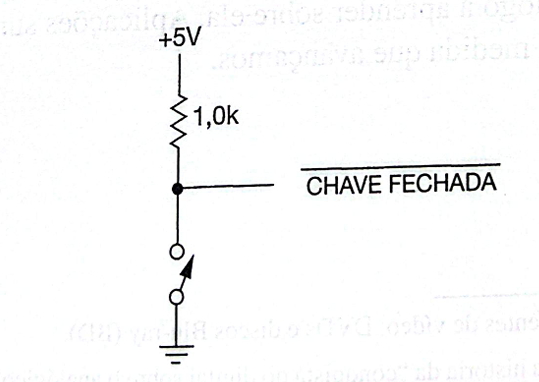
\includegraphics[width=\textwidth]{images/sinal.png}

            \vspace{0.2cm}
            \textbf{Nível Lógico}
        \end{column}
    \end{columns}
\end{frame}